% !TEX root = ../../homo_alg.tex

\newpage
\section{The Derived Category}

\subsection{Derived Categories \& Localization of Categories}

To get better behavior (in the same way that the long exact sequence corrected non exactness), we want to replace modules $M$ by their projective resolutions $\dt{P}$. Note $\dt{P}$ is quasi-isomorphic to $M$. We naturally come to a category where quasi-isomorphic objects are somehow the same, i.e. quasi-isomorphisms are considered isomorphisms. 

Let $\cA$ be an abelian category. Let $\chh(\cA)$ be the (abelian) category of cochain complexes. 

\begin{dfn}[Derived Category]
The derived category $\cD(\cA)$ is a category equipped with a functor $\chh(\cA) \ma{i} \cD(\cA)$ with $i(f)$ an isomorphism for all quasi-isomorphisms $f$ satisfying the universal mapping property: any functor $\chh(\cA) \ma{F} \cC$ transforming quasi-isomorphisms factors uniquely through $\cD(\cA)$. That is, we have a unique $G$ such that the following diagram commutes:
\[
\begin{tikzcd}
\chh(\cA) \arrow{r}{F} \arrow{dr}{i} & \cC \\
& \cD(\cA) \arrow{u}{G}
\end{tikzcd}
\]
Note if such a category exists, it is unique up to isomorphism. 
\end{dfn}

We show the existence of such a category by physically constructing $\cD(\cA)$ by inverting all quasi-isomorphisms. Namely, we will ``localize" $\chh(\cA)$. One should read Gelfand-Manin chapters 3 and 4 for more on this material generally. 

In the proceeding lemma, the category $\cB=\chh(\cA)$ and $S=\{\text{quasi-iso in }\chh(\cA) \subseteq \text{morph }\chh(\cA)\}$. We want to show $\cD(\cA)= S^{-1}\cB$. 

\subsection{Localization of a Category}

Let $\cB$ be a category and let $S$ be a collection of morphisms. Define $S^{-1}\cB$ by $\ob(S^{-1}\cB)\defeq \ob(\cB)$ and morphisms by for each $X \ma{s} Y$ in $S$, adjoin a ``morphism" $X \xleftarrow{s^{-1}} Y$ in $S^{-1}\cB$. Note that $s^{-1}$ is not a morphism in $\cB$ but rather a symbol of sorts. The morphisms in $S^{-1}\cB$ are formal products of morphisms in $\cB$ and these formal inverses $S^{-1}$ for $s \in S$ such that the ``codomain" of each is the ``domain" of the next modulo an equivalence generated by 
\begin{enumerate}[(i)]
\item consecutive morphisms in $\cB$ can be replaced by compositions in $\cB$. 
\item $ss^{-1} \notin S^{-1}S$ can be replaced by $1$.
\item $1s^{-1}=s^{-1}=s^{-1}1$.
\end{enumerate}

so that composition is just concatenation. 

\begin{prop}
\begin{enumerate}[(i)]
\item $S^{-1}\cB$ is a category
\item $i: \cB \to S^{-1}\cB$ given on objects by $\ob: X \mapsto X$ and on morphisms by $f \mapsto f$ is a functor.
\item The category satisfies the universal mapping property for all functors $\cB \ma{F} \cC$ transforming morphisms in $S$ into isomorphism in $\cC$. That is, there is a unique functor $G$ such that 
\[
\begin{tikzcd}
\cB \arrow{r}{F} \arrow{dr}{i} & \cC \\
&  S^{-1}\cB \arrow[dotted]{u}{G}
\end{tikzcd}
\]
\end{enumerate}
\end{prop}

\noindent Proof: The proof of the first two parts is dull and routine verification. For the third, on objects let $G(X)=F(X)$ of $S^{-1}\cB$. Let $G(s_1^{-1}f_1s_2^{-1}f_2 \cdots)=F(s_1)^{-1}F(f_1)F(s_2)^{-1}F(f_2) \cdots$. Note that $i(s)$ in $S^{-1}\cB$ is invertible, $i(s)=s$ so $ss^{-1}=1$ and $s^{-1}s=1$. \qed \\

So we have $\cD(\cA)=S^{-1}(\chh(\cA))$, where $S=\{\text{quasi-iso}\}$. We have a similar description of $S^{-1}\cB$ when $S$ is localizing. 

\begin{dfn}[Localizing Morphisms]
A collection $S \subseteq \text{morph of }\cB$ is localizing if
\begin{enumerate}[(a)]
\item all $1_X \in S$ and $s,t \in S$ implies $st \in S$.
\item for all $f \in S$ with $s \in S$ with the same codomain, there exist $g,t$ with $t \in S$ with a $W$ such that the following square commutes
\[
\begin{tikzcd}
W \arrow{d}{\ep} \arrow{r}{g} & Z \arrow{d}{s} \\
X \arrow{r}{f} & Y 
\end{tikzcd}
\]
\item for $g,t$ as given above, there exist $s,f$ as above.
\item For any $f,g$, there exist $s \in S$ such that $sf=sg$ if and only if there is a $t \in S$ such that $ft=gt$.

\begin{figure}[H] 
   \centering
   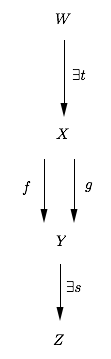
\includegraphics[width=0.5in]{images/p1.png} 
\end{figure}

\end{enumerate}
\end{dfn}

Note the second condition above gives for all $f,s$, there is a $g,t$ such that $ft=sg$ so that in $S^{-1}\cB$, $s^{-1}f=gt^{-1}$ so we can ``rearrange" until all $s$'s (denominators) are on the right and all the $f$'s (numerators) are on the left.

\begin{prop}
Let $S$ be a localizing collection of morphisms. Then $S^{-1}\cB$ can be defined equivalently as 
\begin{enumerate}[(a)]
\item $\ob(S^{-1}\cB)=\ob(\cB)$
\item morphisms $X \to Y$ in $S^{-1}\cB$ are equivalence classes of ``roofs" 

\begin{figure}[H] 
   \centering
   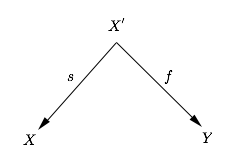
\includegraphics[width=2.5in]{images/p2.png} 
\end{figure}

with $s \in S$, written $(s,f)$. This corresponds to $fs^{-1}$ from the ``old" description of $S^{-1}\cB$. That is, $(s,f) \sim (t,g)$ if and only if there is a commutative diagram


\begin{figure}[H] 
   \centering
   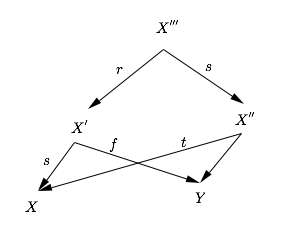
\includegraphics[width=2.5in]{images/p3.png} 
\end{figure}

with $sr \in S$ (but not necessarily $r \in S$). Or that we have the diagram 

\begin{figure}[H] 
   \centering
   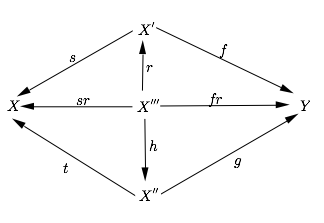
\includegraphics[width=2.5in]{images/p4.png} 
\end{figure}

\item the identity morphism on $X$ is the roof $(1_X,1_X)$.

\item composition of roofs $(s,f)$ and $(t,g)$ is $(st',gf')$ from the diagram

\begin{figure}[H] 
   \centering
   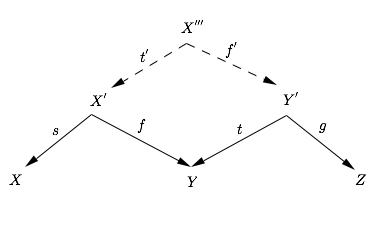
\includegraphics[width=2.5in]{images/p5.png} 
\end{figure}

where the square $f'$ and $t'$ comes from the localizing property. [$gt^{-1}fs^{-1}=gf'(t')^{-1}s^{-1}$]


\item $i: \cB \to S^{-1}\cB$ is given by on objects by $X \mapsto X$ and given on morphisms by $f \mapsto $ the roof $(1,f)$. 

\end{enumerate}
\end{prop}

\noindent Proof: We first show that $\sim$ is an equivalence relation. The reflective and symmetric properties are simple. To see the transitive property, suppose $(s,f) \sim (t,g)$ and $(t,g) \sim (u,e)$, then

\begin{figure}[H] 
   \centering
   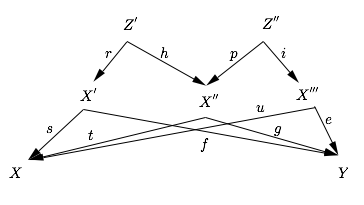
\includegraphics[width=2.5in]{images/p6.png} 
\end{figure}

so we have the commutative diagram as given above with $sr,tp \in S$. By the localizing property, there are $v,k$ with $v \in S$ such that we have

\begin{figure}[H] 
   \centering
   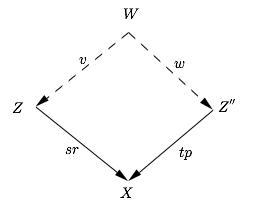
\includegraphics[width=1.5in]{images/p7.png} 
\end{figure}

Now $t=pk=srv=thv$ so there is $Z''' \ma{w} W$ is $S$ such that $pkw=hvw$ so that we have the diagram

\begin{figure}[H] 
   \centering
   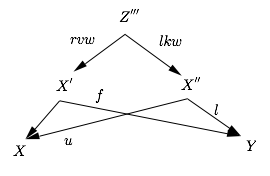
\includegraphics[width=1.5in]{images/p8.png} 
\end{figure}

commuting so $(s,f) \sim (u,e)$. So $\sim$ on roofs is an equivalence relation. Similarly, one can see that composition on roofs is well defined. Furthermore, the category with objects being the objects of $\cB$ and morphisms given by roofs is a category. We show that this category $R$ satisfies the universal mapping property for $S^{-1}\cB$ so that $R=S^{-1}\cB$. 

Given any functor $\cB \ma{F} \cC$ such that $F$ takes morphisms in $S$ to isomorphism in $\cC$, we need to show that there is a unique functor $G$ such that the following diagram commutes
\[
\begin{tikzcd}
\cB \arrow{r}{F} \arrow[hook]{dr}{i} & \cC \\
& R \arrow[dotted]{u}{G}
\end{tikzcd}
\]
where $i$ takes objects to objects via $X \mapsto X$ and on morphisms $f \mapsto (1,f)$. If $G$ exists, then it is unique as $G(X) \defeq G(i(X))=F(X)$ and 
\[
G(f)=G(i(f))=G((s,t))=G((1,s)^{-1}(1,f))=G((1,s))^{-1}G(i(f))=F(s)^{-1}F(f)
\]
Existence of such follows from the above definition. One only need show that it is indeed a functor. \qed \\

\subsection{Homotopy Category, $\cK(\cA)$}

Note that for $\cB=\chh(\cA)$ and $S=\{\text{quasi-iso}\}$, we have $\cD(\cA)\defeq S^{-1}\cB$. Unfortunately, $S$ is \emph{not} a localizing class. But it is if we go ``mod homotopy". 

\begin{dfn}[Homotopy Category]
The homotopy category $\cK(\cA)$ is the category given by $\ob(\cK(\cA))=\ob(\chh(\cA))$, that is cochain complexes, and $\text{morph}(\cK(\cA))$ is the cochain maps modulo homotopy, i.e. $\Hom_{\cK(\cA)}(X,Y)=\Hom_{\chh(\cA)}(X,Y)/\sim$, where $\sim$ is the equivalence $f \sim g$ if and only if $f \simeq g$. 
\end{dfn}

For a complex $K^\cdot$, define $K[x]$ to be $K[n]^i\defeq K^{n+1}$ and $d_{K[x]}=(-1)^n d_k$, called the shift, translation, or suspension. This gives a functor which is an equivalence of categories on $\chh(\cA),\cK(\cA),\cD(\cA)$. For any map $K^\cdot \ma{f} L^\cdot$, we have $C(f)=L^\cdot \oplus K^\cdot[1]$ with mixed differentials and $\cyl(f)=L \oplus K[1] \otimes K$ with differential from the ``tot"

\begin{figure}[H] 
   \centering
   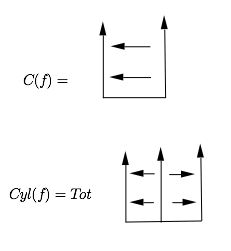
\includegraphics[width=2.5in]{images/p9.png} 
\end{figure}

\begin{lem}
For any cochian map, $K \ma{p} Y$, there is a commutative diagram with exact rows
\[
\begin{tikzcd}
0 \arrow{r} & L \arrow{d}{\alpha} \arrow{r}{i} & C(f) \arrow{r}{p} \arrow{d} & K[1] \arrow{r} & 0 \\
0 \arrow{r} & \cyl(f) \arrow{r} & C(f) \arrow{r} & ? \arrow{r} & 0
\end{tikzcd}
\]
where $\beta(l,k,k')=l+f(K)$ and other maps $\alpha,i,p,\tilde{f},\pi$ are simple inclusions/projections. Furthermore, $\alpha,\beta$ are homotopy equivalent: $\alpha \beta=1_C$ and $\beta \alpha \simeq 1_{C(y)}$ and the pictorial is functional in $f$. 
\end{lem}

\begin{lem}
Let $f,g: K \to L$ with $f \simeq g$, i.e. $f=g$ in $\cK(\cA)$. 
\end{lem}

\noindent Proof: Note that $\cyl(1_K)= \tot(K \leftarrow K \rightarrow K)$. It has two inclusions from $K$: $\alpha(k)=(k,0,0)$ with $\beta \alpha=1, \alpha\beta \simeq 1$ and $\alpha'(k)=(0,0,k)$ with $\beta\alpha'=1,\alpha'\beta\simeq 1$. 

Let $t=\alpha \beta,t'=\alpha'\beta$. Note that $t,t' \in S$ because they are homotopic to 1. Then $tt'=\alpha'\beta\alpha\beta=t'$. Then we have
\[
i(t't)=i(t')=i(t')i(t)=i(t')
\]
as they are isomorphic in $S$ so isomorphic in $\cD(\cA)$. Then we have $i(t)=1$ in $\cD(\cA)$. So
\[
i(\alpha')=i(t)i(\alpha')=i(t\alpha')=i(\alpha\beta\alpha')=i(\alpha)
\]
If $f \simeq g$ via the homotopy $\{s_n: K^{n+1} \to L^n\}$, we construct the map $\gamma=(f,s,g): \cyl(1_k) \to L$. Check that $\gamma$ is a cochain map so that it commutes with differentials (uses the fact that $s$ is a homotopy). Check also that $\gamma \alpha=f$ and $\gamma \alpha'=g$. So 
\[
i(f)=i(\gamma\alpha)=i(\gamma)i(\alpha)=i(\gamma)i(\alpha')=i(g)
\]

\begin{figure}[H] 
   \centering
   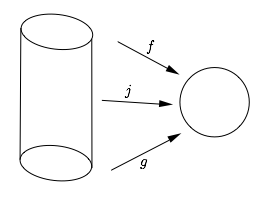
\includegraphics[width=2.5in]{images/p10.png} 
\end{figure}

So we are getting a mapping cylinder to some object so that the map of the top and bottom are the same somehow. \qed \\

\begin{thm}
\begin{enumerate}[(i)]
\item The functor 
\[
\begin{tikzcd}
i: \chh(\cA) \arrow{r} \arrow{dr}{\pi} & \cD(\cA)=S^{-1}\chh(\cA) \\
& \cK(\cA) \arrow[dotted]{u}{\exists}
\end{tikzcd}
\]
factors through $\cK(\cA)$. 

\item $\cD(\cA)=S^{-1}\cK(\cA)$ with $S=\{\text{equiv classes of quasi-iso}\}$. Note that if two morphisms are in the same equivalence class and one is a quasi-iso then the other is.

\item $S$ is a localizing class in $\cK(\cA)$. So you can describe $\cD(\cA)$ as ``roofs of maps modulo homotopy". 
\end{enumerate}
\end{thm}

\noindent Proof: The first part is obvious from the proceeding lemma. For the second part, this is easy from the universal mapping property of localization $R \to S^{-1}R$. For the third part, we need show that $S=\{\text{quasi-iso}\}$ is a localizing class in $\cK(\cA)$. Note that $1_X \in S$ and that if $f,g$ are quasi-iso then $fg$ is a quasi-iso. Then given $f,s$ with $s$ a quasi-iso, we need to find $g,t$ with $t$ quasi-iso so that 

\begin{figure}[H] 
   \centering
   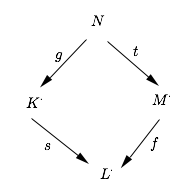
\includegraphics[width=1.5in]{images/p11.png} 
\end{figure}

Form the cone of $s$. Compose $i$ with $f$ to form the cone of $if$:
\[
\begin{tikzcd}
C(if)[-1] \arrow[dotted]{d} \arrow{r}{t} & M \arrow{d}{f} \arrow{r}{if} & C(s) \arrow{d}{=} \arrow{r} & C(if) \\
K \arrow{r}{s} & L \arrow{r}{i} & C(s) & 
\end{tikzcd}
\]
where $t$ is the usual projection to $M$ and $g$ is the usual projection to $K$. The square does not commute in $\chh(\cA)$ as $f(m) \neq s(k)$. But it is commutative up to homotopy. $ft \simeq sg$ via the homotopy $\sigma(m,l,k)=l^{n-1}$. It is routine to check that this works. Hence, the diagram commutes in $\cK(\cA)$. It is also easy to check that this is a quism and that the quism for the long exact sequence of $C(s)$ is exact so that $t$ is a queasy. Similarly, $g,t$ given as above shows there is a $f,s$ as above. For the final part, suppose 
\[
\begin{tikzcd}
K \arrow[yshift=1ex]{r}{f} \arrow[yshift= -1ex]{r}{g} & L \arrow{r}{s} & M
\end{tikzcd}
\]
with $s \in \cK(\cA)$ with $sf=sg$ in $\cK(\cA)$, i.e. $sf \simeq sg$. Let $\sigma: K \to L[-1]$ be a homotopy 
\[
\begin{tikzcd}
C(s)[-1] \arrow{d}{=} & K \arrow{d}{f-g} \arrow{l}{h} & C(h)[-1] \arrow{l}{t} \\
C(s)[-1] \arrow{r}{p} & L \arrow{r}{s} & M
\end{tikzcd}
\]
Define $h$ by $h(k)=(\sigma(k),(f-g)(k))$. The square commutes. Take the cone of $h$ then $(f-g)t=pht=0$ in $\cK(\cA)$ since $ht \simeq 0$ and $s$ is a quism so that there is a long exact sequence giving $C(s)$ is exact so that by the long exact sequence so that $t$ is a quism. So $ft \simeq gt$ so that they are equal in $\cK(\cA)$ so that $t \in S$. \qed \\

\begin{cor}
For any $K \ma{f} L$ in $\chh(\cA)$, $f=0$ in $\cD(\cA)$ if and only if there is a quism $L \ma{s} M$ such that $sf \simeq 0$ in $\chh(\cA)$ (that is, $f=0$ in $\cK(\cA)$). 
\end{cor}

\noindent Proof: Exercise. (By the theorem, going via $\cK(\cA)$, $\cD(\cA)=S^{-1}\cK(\cA)$ and $S$ is a localizing collection in $\cK(\cA)$ so the maps are roofs). \qed \\

\subsection{Distinguished Triangles}

As $\cD(\cA)$ is an additive category (see the book) but is almost never abelian, we can not talk about short exact sequence and homology. We need to find a replacement for short exact sequences. The replacement will be something with similar behavior: distinguished triangles.

\begin{dfn}[(Distinguished) Triangles]
A triangle in a category of complex is a diagram
\[
K^\cdot \ma{} L^\cdot \ma{} M^\cdot \ma{w} K^\cdot[1]
\]
notice how this can be arranged in a triangle (ignoring shift). In fact, we also have
\[
\cdots K \ma{u} L \ma{v} M \ma{w} K[1] \ma{u[1]} L[1] \ma{} \cdots 
\]
This is \emph{not} exact as we cannot even talk about exactness. A morphism of triangles is a commutative diagram 
\[
\begin{tikzcd}
K \arrow{d}{f} \arrow{r} & L \arrow{d}{g} \arrow{r} & M \arrow{d}{h} \arrow{r} & K[1] \arrow{d}{f[1]} \\
K' \arrow{r} & L' \arrow{r} & M' \arrow{r} & K'[1]
\end{tikzcd}
\]
It is an isomorphism of triangles if $f,g,h$ are isomorphisms in that category. A distinguished triangle is one isomorphic to
\[
K \ma{\tilde{f}} \cyl(f) \ma{\pi} C(f) \ma{p} K[1]
\] 
for some $K \ma{f} L$. That is, we have an isomorphism of triangles
\[
\begin{tikzcd}
K \arrow{d}{=} \arrow{r}{\tilde{f}} & \cyl(f) \arrow{r}{\pi} \arrow{d}{\beta} & C(f) \arrow{d}{=} \arrow{r}{p} & K[1] \arrow{d}{=} \\
K \arrow{r}{f} & L \arrow{r}{i=\pi\alpha} & C(f) \arrow{r}{p} & K[1]
\end{tikzcd}
\]
with $\beta$ a homotopy equivalence so that the diagram commutes up to homotopy. $i \beta=\pi \alpha \beta \simeq \pi 1 =\pi$? 
\end{dfn}

Let us now see the relation to the short exact sequences of $\chh(\cA)$. 

\begin{prop}
An exact sequence
\[
0 \ma{} K \ma{f} L \ma{g} M \ma{} 0
\]
in $\chh(\cA)$ is an isomorphism to a short exact sequence that can be extended to a distinguished triangle in $\cK(\cA)$ or $\cD(\cA)$. Conversely, every distinguished triangle is isomorphic to one that is an extension of a short exact sequence in $\chh(\cA)$. 
\end{prop}

\noindent Proof ($\cD(\cA)$): The following diagram commutes
\[
\begin{tikzcd}
0 \arrow{r} & K \arrow{d}{=} \arrow{r}{f} & L \arrow{r}{g} & M \arrow{r} & 0 \\
0 \arrow{r} & K \arrow{r} & \cyl(f) \arrow{u}{\beta} \arrow{r} & C(f) \arrow{r} & 0 
\end{tikzcd}
\]
where $\beta$ is the usual map $\beta(l,k,k')=l+f(K)$, $\gamma(l,k)=g(l)$ and has exact rows. Also, $\beta$ is a homotopy equivalence (in $\cK(\cA)$, we need to show that $\gamma$ is a homotopy equivalence, in $\cD(\cA)$ need to show that $\gamma$ is a quism). By the long exact sequence on homology and the Five Lemma, $h(\gamma)$ is an isomorphism for all $n$ so that $\gamma$ is a quism. So then it is an isomorphism in $\cD(\cA)$ and the bottom row now extends to a distinguished triangle
\[
K \ma{} \cyl(f) \ma{} C(f) \ma{} K[1]
\]
Conversely, given a distinguished triangle clearly
\[
0 \ma{} K \ma{} \cyl(f) \ma{} C(f) \ma{} 0
\]
is a short exact sequence in $\chh(\cA)$. \qed \\

\begin{prop}[Long Exact Sequences]
If $K \ma{} L \ma{v} M \ma{w} K[1]$ is a distinguished triangle in $\cD(\cA)$, then the induced sequence 
\[
\cdots \ma{} H^i(M[-1]) \ma{} H^i(K) \ma{H(w)} H^i(L) \ma{H(v)} H^i(M)\ma{H(w)} H^i(K[1]) \ma{} \cdots
\]
is exact. 
\end{prop} 

\noindent Proof: The distinguished triangle is isomorphic to the triangle
\[
K \ma{u} L \ma{i} C(u) \ma{p} K[1]
\]
so the long exact sequence is really
\[
\cdots \ma{} H^i(K) \ma{H(u)} H^i(L) \ma{H(l)} H^i(C(u)) \ma{H(p)} H^i(K[1])=H^{i+1}(K) \ma{} \cdots
\]
which is exactly the long exact sequence you get from the cone short exact sequence
\[
0 \ma{} L \ma{} C(u) \ma{} K[1] \ma{} 0
\]
so we get $H(u)=\delta$ from the long exact sequence. \qed \\

\subsection{Rotating Triangles}

Can we rotate any triangle but does this preserve distinguished triangles?

\begin{prop}
Distinguished triangles are preserved under rotation.
\end{prop}

\noindent Proof: It is enough to show for a rotation in one direction and then the rest follows by induction. Without loss of generality, assume we rotate the triangle counter-clockwise. Up to isomorphism, a distinguished triangle of the form
\[
K \ma{f} L \ma{i} C(f) \ma{p} K[1]
\]
under rotation is
\[
C(f)[-1] \ma{} K \ma{f} L \ma{} C(f)
\]
is $L$ the cone of the first map?
\[
\begin{tikzcd}
C(f)[-1] \arrow{d}{=} \arrow{r} & K \arrow{d}{=} \arrow{r}{f} & L \arrow{r} & C(f) \arrow{d}{=} \\
C(f)[-1] \arrow{r}{p[-1]} & K \arrow{r} & \cyl(f)=C(p[-1]) \arrow{r}{\pi} & C(f)
\end{tikzcd}
\]
\qed \\

\subsection{Ext \& $\cD(\cA)$}

We have an obvious functor $\cA \ma{i} \cD(\cA)$ given by $X$ maps to the complex $\cdots \to 0 \to X \to 0 \to \cdots$, where $X$ is in position (degree or index) 0. This is called the ``stalk" of $X$ and is denoted $X[0]$ and takes morphisms to morphisms. But in $\cD(\cA)$, $i(X)=X[0]$ is isomorphic to any complex quasi-isomorphic to it. For example, $X$ is quasi-iso to a projective resolution of it. We call any complex $K$ with $H_i(K)=0$ for all $i \neq 0$ a $H^0$-complex. 

\begin{prop}
The functor $i: \cA \to \cD(\cA)$ gives an equivalence of categories of $\cA$ with the full subcategory of $\cD(\cA)$ consisting of all $H^0$-complexes. 
\end{prop}

\noindent Proof: By definition, $i$ is injective on objects. To see that $i$ is onto modulo isomorphism, if $K$ is an $H^0$-complex, there are quasi-isomorphisms as follows:
\[
\begin{tikzcd}
\cdots \arrow{r} & K^{-2} \arrow{r} & K^{-1} \arrow{r} & K^0 \arrow{r}{d_0} & K^1 \arrow{r} & K^2 \arrow{r} & \cdots \\
\cdots \arrow{r} & K^{-2} \arrow{r} \arrow{u}{1} & K^{-1} \arrow{r} \arrow{u}{1} & \ker d_0 \arrow{u} & 0 \arrow{u} & 0 \arrow{r} \arrow{u} & \cdots 
\end{tikzcd}
\]
where we can extend $\ker d_0 \to H^0(K)=\ker d_0/\im d^{-1}$. This is called the ``soft truncation of $K$". Why? We have cut off the sequence gently so that the homology does not change. So this is isomorphic to $K$ in $\cD(\cA)$, $i(H^0(\cK))$ the stalk complex. To see $i$ is fully faithful, oe only need show that $\Hom_{\cA}(X,Y) \cong \Hom_{\cD(\cA)}(i(X),i(Y))$. \qed \\

\begin{dfn}[Ext]
For an object $X \in \cA$, let $X[-i]$ denote the complex with $X$ in position $i$ and 0 elsewhere. For $X,Y \in \cA$, define
\[
\Ext_{\cA}^i(X,Y) \defeq \Hom_{\cD(\cA)}(X[0],Y[i])
\]
\end{dfn}

\begin{rem}
\begin{enumerate}[(i)]
\item $\Ext_{\cA}^0(X,Y)\defeq \Hom_{\cD(\cA)}(i(X)=X[0],i(Y)=Y[0])=\Hom_{\cA}(X,Y)$ so that $\Ext_{R-\text{mod}}^0(X,Y)=\Hom_{R-\text{mod}}(X,Y)=\Hom_R(X,Y)$.
\item Since the shift $[k]$ gives an equivalence of categories on $\chh(\cA),\cK(\cA),\cD(\cA)$ (as $[-k]$ is an inverse), we get that $\Ext_{\cA}^i(X,Y)\defeq \Hom_{\cD(\cA)}(X[0],Y[i])\cong \Hom_{\cD(\cA)}(X[k],Y[i+k])$ for any $k \in \Z$. We can use this to define a composition $\Ext^i(X,Y) \times \Ext^j(Y,Z) \to \Ext^{i+j}(X,Z)$ so that $\oplus \Ext^i(X,X)$ is a graded ring. This is often used in Representation Theory.
\item $\Ext_{\cA}^i(X,Y)=0$ for $i<0$.To see this, if $i<0$ and $\varphi \in \Hom_{\cD(\cA)}(X[0],Y[i])$, then $\varphi=s^{-1}f$ a roof. 

\begin{figure}[H] 
   \centering
   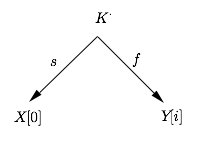
\includegraphics[width=1.5in]{images/p12.png} 
\end{figure}

Let $L$ be a soft truncation of $K^\cdot$ at degree $-i-1$ (note that $K$ is quism to $X[0]$ via $s$). It is easy to check

\begin{figure}[H] 
   \centering
   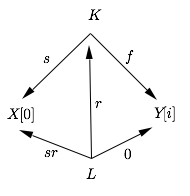
\includegraphics[width=1.5in]{images/p13.png} 
\end{figure}

commutes up to homotopy and $s,r$ are quisms. So in $\cD(\cA)$, we have $(s,f) \sim (sr,0)$ to $Y[i]$ for $i<0$. 

\item We have a relation to the Yoneda Extension: for $i \geq 0$, we look at the two definitions of $\Ext^i(X,Y)$. The ``classic" definition gives any exact sequence
\[
0 \ma{} Y \ma{} K^{-i+1} \ma{} \cdots \ma{} K^0 \ma{\ep} X \to 0
\]
Call this sequence $\hat{K}$. We have a roof

\begin{figure}[H] 
   \centering
   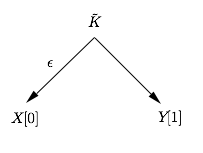
\includegraphics[width=1.5in]{images/p14.png} 
\end{figure}

i.e. an element of $\Ext_{\cA}^i(X,Y)=\Hom_{\cD(\cA)}(X[0],Y[i])$. It turns out to be all such elements of $\Ext_{\cA}^i(X,Y)$.


\item Let $I=$ the full subcategory of $\cA$ of injective modules. Consider $\cK^+(I)$, complexes bounded below, of injective objects with morphisms being composition. Then the obvious functor $\cK^+(I) \to \cD^+(\cA)$ is an equivalence of categories. This is proven on 179-183 of GM. We have a similar statement for the category of projectives $\cK^-(P) \to \cD^{-}(\cA)$. In the proof, one also gets if $X \in \chh^-(P)$ or $Y \in \chh^{-}(I)$, then $\Hom_{\cK(\cA)}(X,Y) \cong \Hom_{\cD(\cA)}(X,Y)$ as sets. The reveres direction here is exciting. It was first used to define $\Ext$ if the first component projective or second injective we are able to compute it. This gives a computation of $\Ext$ for objects $X,Y \in \cA$. So we have a new definition
\[
\begin{split}
\Ext_{\cA}^i(X,A) &\defeq \Hom_{\cD(\cA)}(X[0],Y[i]) \\
&=\Hom_{\cD(\cA)}(\dt{P},Y[i]) \\
&=\Hom_{\cK(\cA)}(\dt{P},Y[i]) \\
&=\Hom_{\chh(\cA)}(\dt{P},Y[i])/\text{homotopy}
\end{split}
\]

\item We have derived functors of $F$, $RF,LF$. See III.6 of GM. These are similar to $\Ext,\Tor$ and the class $L_nF$ and $R_nF$ but don't take homology. $R\Hom(X,Y) \defeq \Hom(\dt{P},Y)$ as a complex in $\chh(\cA)$ or $\cK(\cA)$ or $\cD(\cA)$ which are nicer to work with then $H^i$. 

\end{enumerate}
\end{rem}



